\setAuthor{Jaan Kalda}
\setRound{lahtine}
\setYear{2018}
\setNumber{G 10}
\setDifficulty{10}
\setTopic{TODO}

\prob{Pulk}
\begin{wrapfigure}[7]{r}{0.4\textwidth}
	\vspace{-25pt}
	\begin{center}
		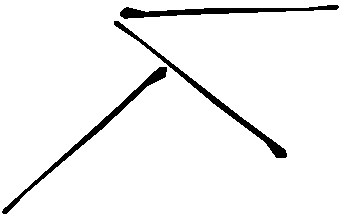
\includegraphics[width = 0.4\textwidth]{2018-lahg-10-yl.pdf}
	\end{center}
\end{wrapfigure}

Õhkuvisatud pulga lendu filmiti liikumatu videokaamera abil ja kahe võrdse intervalli tagant võetud kolm kaadrit kopeeriti juuresolevale joonisele (suuremalt lisalehel). On teada, et esimese ja viimase kasutatud kaadri vahele jäänud ajavahemiku jooksul jäi pulga pöördenurk väiksemaks täispöördest. Pulk pöörles joonise tasandis, pulga pikkus oli $L=\SI{1.0}m$ ja kaadri lühem külg on täpselt vertikaalne; raskuskiirendus $g=\SI{9.8}{m/s^2}$. Kui kaugel pulga jämedamast otsast asub selle massikese? Kui pikk oli esimese ja viimase kaadri vaheline ajavahemik?


\hint

\solu
Esimese ja teise kaadri-intervalli jooksul pöördus pulk sama nurga võrra, see tähendab, et peaaegu horisontaalne pulga asend peab pärinema keskmiselt kaadrilt ja ülejäänud asendid on ca $\pm 140^\circ$ võrra pööratud. Üldsust kitsendamata võime eeldada, et vasak alumine asend vastab esimesele kaadrile (kui see vastab tegelikult viimasele, siis vaatleme pulga liikumist tagurpidi kulgevas ajas). Jooniselt teeme kindlaks, et esimese kaadriintervalli jooksul nihkus pulga peenem ots horisontaalsihis paremale ca $p_1=\SI{155}{cm}$ võrra ja jämedam ots --- $j_1=\SI{-20}{cm}$  võrra. Et teatud pulga punkti horisontaalne nihe esimese kaadriintervalli jooksul $s_1$ on lineaarne funktsioon selle punkti kaugusest $x$ pulga jämedamast otspunktist, siis $s_1=p_1\frac xL+j_1(1-\frac xL)$, kus $L$ tähistab pulga pikkust. Analoogselt leiame nihked teise kaadriintervalli jaoks $p_2=\SI{-105}{cm}$ ja $j_2=\SI{75}{cm}$ ning $s_2=p_2\frac xL+j_2(1-\frac xL)$. Et massikeskme horisontaalne kiiruskomponent ei muutu, siis $s_1=s_2$, millest $\frac xL(p_1-p_2+j_2-j_1)=j_2-j_1$, st $x=L\frac{95}{355}\approx \SI{27}{cm}$.

Teeme nüüd jooniselt kindlaks massikeskme vertikaalsihilised nihked: $v_1=\SI{45}{cm}$ ja $v_2=\SI{-50}{cm}$.
Olgu kaadriintervall $\tau$; massikeskme keskmine kiirus esimese kaadriintervalli jooksul oli $v_1/\tau$ ja teise jooksul --- $v_2/\tau$ ning muutus - $(v_2-v_1)/\tau= -g\tau$, seega $\tau=\sqrt{(v_1-v_2)/g}\approx \SI{0.31}s$.
\probend